% Asset ID: AS1TrigonometricRatiosTIKZ-008
% Source: P1-Chp9 pp.37-38
% Related section: Transformations
% Purpose: Four transformed trig graph notes
\documentclass[tikz,border=8pt]{standalone}
\usepackage{amsmath}
\usetikzlibrary{angles,quotes,calc,arrows.meta}
\begin{document}
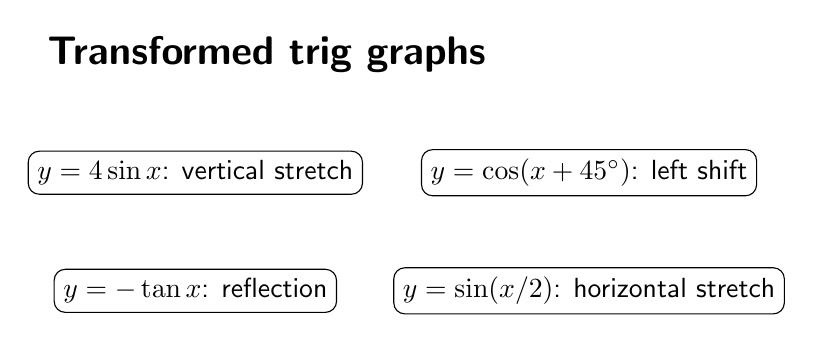
\begin{tikzpicture}[scale=1.0, every node/.style={font=\sffamily}]
\node[font=\sffamily\bfseries\Large, anchor=west] at (0,5) {Transformed trig graphs};
\node[draw,rounded corners] at (2,3.5) {$y=4\sin x$: vertical stretch};\node[draw,rounded corners] at (7,3.5) {$y=\cos(x+45^\circ)$: left shift};\node[draw,rounded corners] at (2,2) {$y=-\tan x$: reflection};\node[draw,rounded corners] at (7,2) {$y=\sin(x/2)$: horizontal stretch};
\end{tikzpicture}
\end{document}
